\documentclass[10pt,a4paper,oneside]{article}
\usepackage{ctex} % 中文支持
\usepackage{titling} % 标题格式定制
\usepackage{lipsum} % 示例文本
\usepackage{titlesec} % 标题格式定制
\usepackage{amsmath,amsthm,amssymb,floatrow}
\usepackage{lmodern}
\usepackage{geometry}
\usepackage{graphicx,float,subfigure,ctex}
\geometry{left=2.5cm,right=2.5cm,top=2.54cm,bottom=2.0cm}
\DeclareGraphicsExtensions{.pdf,.jpeg,.png,.jpg}
\pagestyle{empty}

% 设置标题格式
\titleformat{\section}{\centering\Large\bfseries}{\thesection}{1em}{}
\titleformat{\subsection}{\centering\large\bfseries}{\thesubsection}{1em}{}
\titleformat{\subsubsection}{\centering\normalsize\bfseries}{\thesubsubsection}{1em}{}

% 调整标题位置
\setlength{\droptitle}{-4cm}

\begin{document}

\title{\huge{\textbf{2024秋数值代数-实验报告\#2}}}
\author{姓名:\underline{李奕萱} \hspace{1cm}学号:\underline{PB22000161} }
\date{\today}

\maketitle

运行环境:[win11,vscode,py3]

\section*{实验内容与要求}


分别编写~Newton 迭代法 (通常也称 Newton-Raphson 迭代法)
$$x_{n+1}=x_n-\frac{f(x_n)}{f'(x_n)}$$
和 %Damped-Newton (DN) 迭代
霍氏迭代法
%\begin{center}
%\end{center}
   % $x_{k+1}=x_K-\tau\frac{f(x_k)}{f'(x_k)}$,(其中阻尼参数$\tau$: 0 <$\tau$< 1)
 $$x_{n+1}= x_n - \frac{2f(x_n)f'(x_n)}{2f'(x_n)f'(x_n) - f(x_n)f''(x_n)}, , n=0,1,2,\cdots$$
的通用程序, 并利用它们对如下非线性方程
$$ f(x)\triangleq{arctan(x)}+2xsin(x) - 1.1958 =0$$
求根. %取阻尼参数$\tau$=0.55,
计算中的停止条件为~$|f(x_n)|<10^{-9}$~或迭代步数~$n>10^4$~(可视为迭代失败).
{\bf 提示}:编程前分别手算出~$f'(x), f''(x)$。

\begin{itemize}
    \item 列表给出两种迭代方法在初始点 $x_0$ 依次取值~-55, -40, -30, -20, -8, 0, 10, 22, 30, 40, 50~时的迭代步数
    (若迭代步数超过1万步,可视为迭代失败)
    以及相应的数值解~$x_n$~(保留小数点后6位; 迭代失败时无需给出);
    \item 比较并分析两种方法的优劣,给出合理的算法分析并作实验小结。
\end{itemize}
\clearpage

\section{数值结果(列表或作图)}
函数~$f(x)$~图像参见图1; 计算结果参见图2.

\begin{figure}[H]
  \centering
  \caption{$f(x)$图像}
  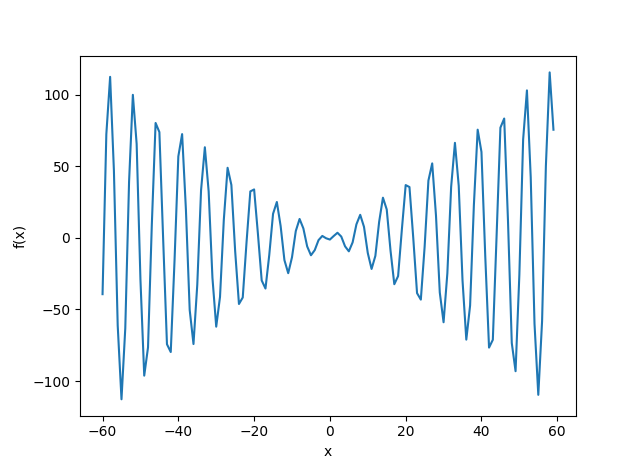
\includegraphics[width=0.8\textwidth]{Figure_1.png}
\end{figure}

\begin{figure}[H]
  \centering
  \caption{实验结果: 误差精度~$\varepsilon = 10^{-9}$, 最大迭代步数为$10^4$}
  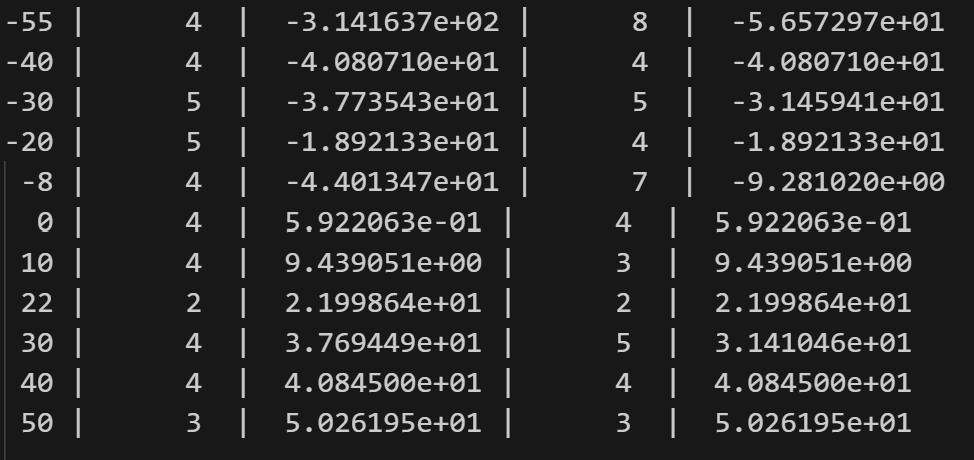
\includegraphics[width=0.8\textwidth]{jg.png}
\end{figure}


{\bf 其中第一列为初始x值,第二列第三列为牛顿迭代法的迭代步数和
计算结果,第四列第五列为霍氏迭代法的迭代步数和计算结果。}

\section{算法分析}
从表一中可以观察到:
\begin{itemize}
    \item 在-55,-30,-8,30时二者有较明显的差距。
    \item 在-20,10时,虽然结果一样,但是牛顿迭代法迭代次数要大于霍氏迭代法。
    \item 在-55,-8,30时,虽然相较于牛顿迭代法距离初始值更近,但是霍氏迭代法迭代次数更多。
\end{itemize}



\section{实验小结}
在本次数值实验中,我们分别测试了两种非线性方程求根的计算方法,
发现了在方程有多个解时,两种结果得到的答案不一定相同,
同时体会了解方程
算法的选择的重要性。最终得到以下结果:

~Newton~迭代法的优点:

\begin{itemize}
    \item 只需要求一阶导数,计算成本更低;
    \item 二次收敛,收敛速度快;
    \item 适用范围广,只要可以求导数都可进行计算。
\end{itemize}

缺点是:

\begin{itemize}
  \item 如果初始值不够靠近解,可能导致发散或找不到我们想要的根;
  \item 若某点导数为零,可能不适用;
  \item 牛顿迭代法通常只保证局部收敛,当初始值差距过大时,容易找不到解。
\end{itemize}

霍氏迭代法的优点:

\begin{itemize}
  \item 相比牛顿迭代法收敛速度更快,同样结果所需迭代次数更少;
  \item 在某些情况下,霍氏迭代法比牛顿迭代法更稳定,因为它减少了高阶导数的影响;
\end{itemize}

缺点是:

\begin{itemize}
  \item 需要求二阶导数,计算成本更高,且限制更大。
  \item 与牛顿迭代法一样,霍纳迭代法也具有局部收敛性,意味着如果初始猜测不适当,可能不会收敛到正确的根。
\end{itemize}

\end{document}
